\documentclass[11pt]{article}

% ---------- Packages ----------
\usepackage[margin=1in]{geometry}
\usepackage{amsmath, amssymb}
\usepackage{graphicx}
\usepackage{fancyhdr}
\usepackage{float}
\usepackage{listings}
\usepackage{xcolor}

\lstset{
    language=Matlab,
    basicstyle=\ttfamily\small,
    breaklines=true,
    breakatwhitespace=false,
    columns=fullflexible,
    showstringspaces=false,
    tabsize=4
}

% ---------- Paragraph Formatting ----------
\setlength{\parindent}{0pt}
\setlength{\parskip}{0.5em}

% ---------- Header ----------
\pagestyle{fancy}
\fancyhf{}
\lhead{ASEN 5090 Introduction    GNSS}
\rhead{Justin Le}
\cfoot{\thepage}

% ---------- Document ----------
\begin{document}

% ---------- Title ----------
\begin{center}
    {\Large \textbf{Fall 2026 Midterm}}\\[0.5em]
    {\large ASEN 5090 Introduction to GNSS}\\[0.5em]
    Justin Le\\
    \today
\end{center}

\vspace{1em}

\section*{Exam Info}
\subsection*{Start Date \& Time}
\hspace*{2em}October 23rd, 2026, 1130
\subsection*{End Date \& Time}

\subsection*{Honor Code}
\textit{On my honor, as a University of Colorado Boulder student, I have followed all of the above instructions
and have neither given nor received unauthorized assistance on this work.}


\centerline{Justin Le, October 23rd, 2026}

\newpage
\section*{Problem 1:}
\subsection*{(a.)}
\hspace*{2em}Because both orbits are circular, we can simply use the formula to solve for the orbital velocity of a satellite in a circular orbit with the gravitational constant for Earth, $\mu_E =  398600.5~\mathrm{km^3/s^2}$,
\begin{gather*}
v = \sqrt{\frac{\mu_E}{r}},~r_{GPS} = 26560~\mathrm{km},~r_{LEO} = 7180~\mathrm{km} \\
\\
\text{Solving for each radius of the respective satellites,}\\
\boxed{v_{GPS} = 3.87~\mathrm{km/s}} \\
\boxed{v_{LEO} = 7.45~\mathrm{km/s}}
\end{gather*}
\subsection*{(b.)}
\hspace*{2em}The minimum geometrical range for a satellite with some observer on the equator of the Earth would be when the satellite directly passes overhead the observer at an elevation of $el = 90^\circ$ we can then account for this with the geometrical range equation,
\begin{gather*}
R = \sqrt{R_E^2(\sin^2{el-1}) + R_{sat}^2} - R_E \sin{el},~el=90^\circ \\
\\
\text{We use the corresponding ranges from LEO and GPS to solve,} \\
\boxed{\rho_{GPS min} = 20180~\mathrm{km}} \\
\boxed{\rho_{GPS min} = 800~\mathrm{km}}
\end{gather*}

\subsection*{(c.)}
\hspace*{2em}To find the maximum geometrical range for which the satellite is visible, we want to account for when the elevation is $0^\circ$ for each satellite. Using the same equation in part b but with an elevation of $el=0^\circ$,
\begin{gather*}
\boxed{\rho_{GPS max} = 2.578\times10^4~\mathrm{km}} \\
\boxed{\rho_{GPS max} = 3.294\times10^3~\mathrm{km}}
\end{gather*}

\subsection*{(d.)}
\hspace*{2em}When assuming a non rotating Earth, perfect satellite and user clocks, and clear view all the way down,the doppler shift of a satellite transmitting at the minimum geometrical range would be $0~\mathrm{Hz}$ for both satellites. Because doppler frequency is dependent on the range rate of the satellite, at this point the range would be a minimum which leads to zero doppler shift.  

\subsection*{(e.)}
\hspace*{2em}With similar assumptions listed in part d, when calculating the doppler shift at the maximum geometrical range, the doppler shift will be inherently bounded by the orbital speed of the satellite, which will be different for each GPS and LEO satellite scenario. Finding the doppler shift at some elevation of 0 we use,
\begin{gather*}
f_D = \frac{v_{sat}}{c} \frac{R_{obs}}{R_{sat}} f_{carrier} \\
\\
\text{Substituing the corresponding velocities found in part a, the geometric ranges in part b, and the given carrier frequencies of each satellite, we find that,} \\
\boxed{f_{D GPS} = 4.87~\mathrm{kHz} = 4.87\times10^3~\mathrm{Hz}} \\
\boxed{f_{D LEO} = 176.55~\mathrm{Hz} = 176.55\times10^3~\mathrm{Hz}}
\end{gather*} 

\begin{table}[h!]
\centering
\renewcommand{\arraystretch}{2}
\begin{tabular}{|p{8cm}|p{4cm}|p{4cm}|p{4cm}|}
\hline
& GPS & LEO \\ \hline

Satellite speed (magnitude of velocity)
& $3.87~\mathrm{km/s}$ & $7.45~\mathrm{km/s}$ \\ \hline

Minimum geometrical range
& $20180~\mathrm{km}$ & $800~\mathrm{km}$ \\ \hline

Maximum geometrical range for which the satellite is visible
& $2.578\times10^4~\mathrm{km}$ & $3.294\times10^3~\mathrm{km}$ \\ \hline

Doppler shift at minimum geometrical range
& $0~\mathrm{Hz}$ & $0~\mathrm{Hz}$ \\ \hline

Doppler shift at maximum geometrical range
& $4.87\times10^3~\mathrm{Hz}$ & $176.55\times10^3~\mathrm{Hz}$ \\ \hline

\end{tabular}
\caption{GPS vs LEO}
\label{tab:GPSvLEO}
\end{table}

\subsection*{(f.)}
\hspace*{2em}When comparing the pseudorange ionospheric delays between the two satellites, we can use the equation that approximates the first order terms which models the ionospheric effects due to TEC,
\begin{gather*}
I_{\rho} = \frac{40.3 TEC}{f_{carrier}^2}
\end{gather*} 
\hspace*{2em}When both satellites are directly overhead at zenith, the TEC at LEO satellite is at zenith would be smaller than the TEC at the GPS satellite. Taking that into account and also the fact that the frequency for the LEO sat is greater than the GPS satellites' carrier frequency, the ionospheric effect of the LEO sat should be much less than the GPS satellite's.

\subsection*{(g.)}
\begin{figure}[H]
    \centering
    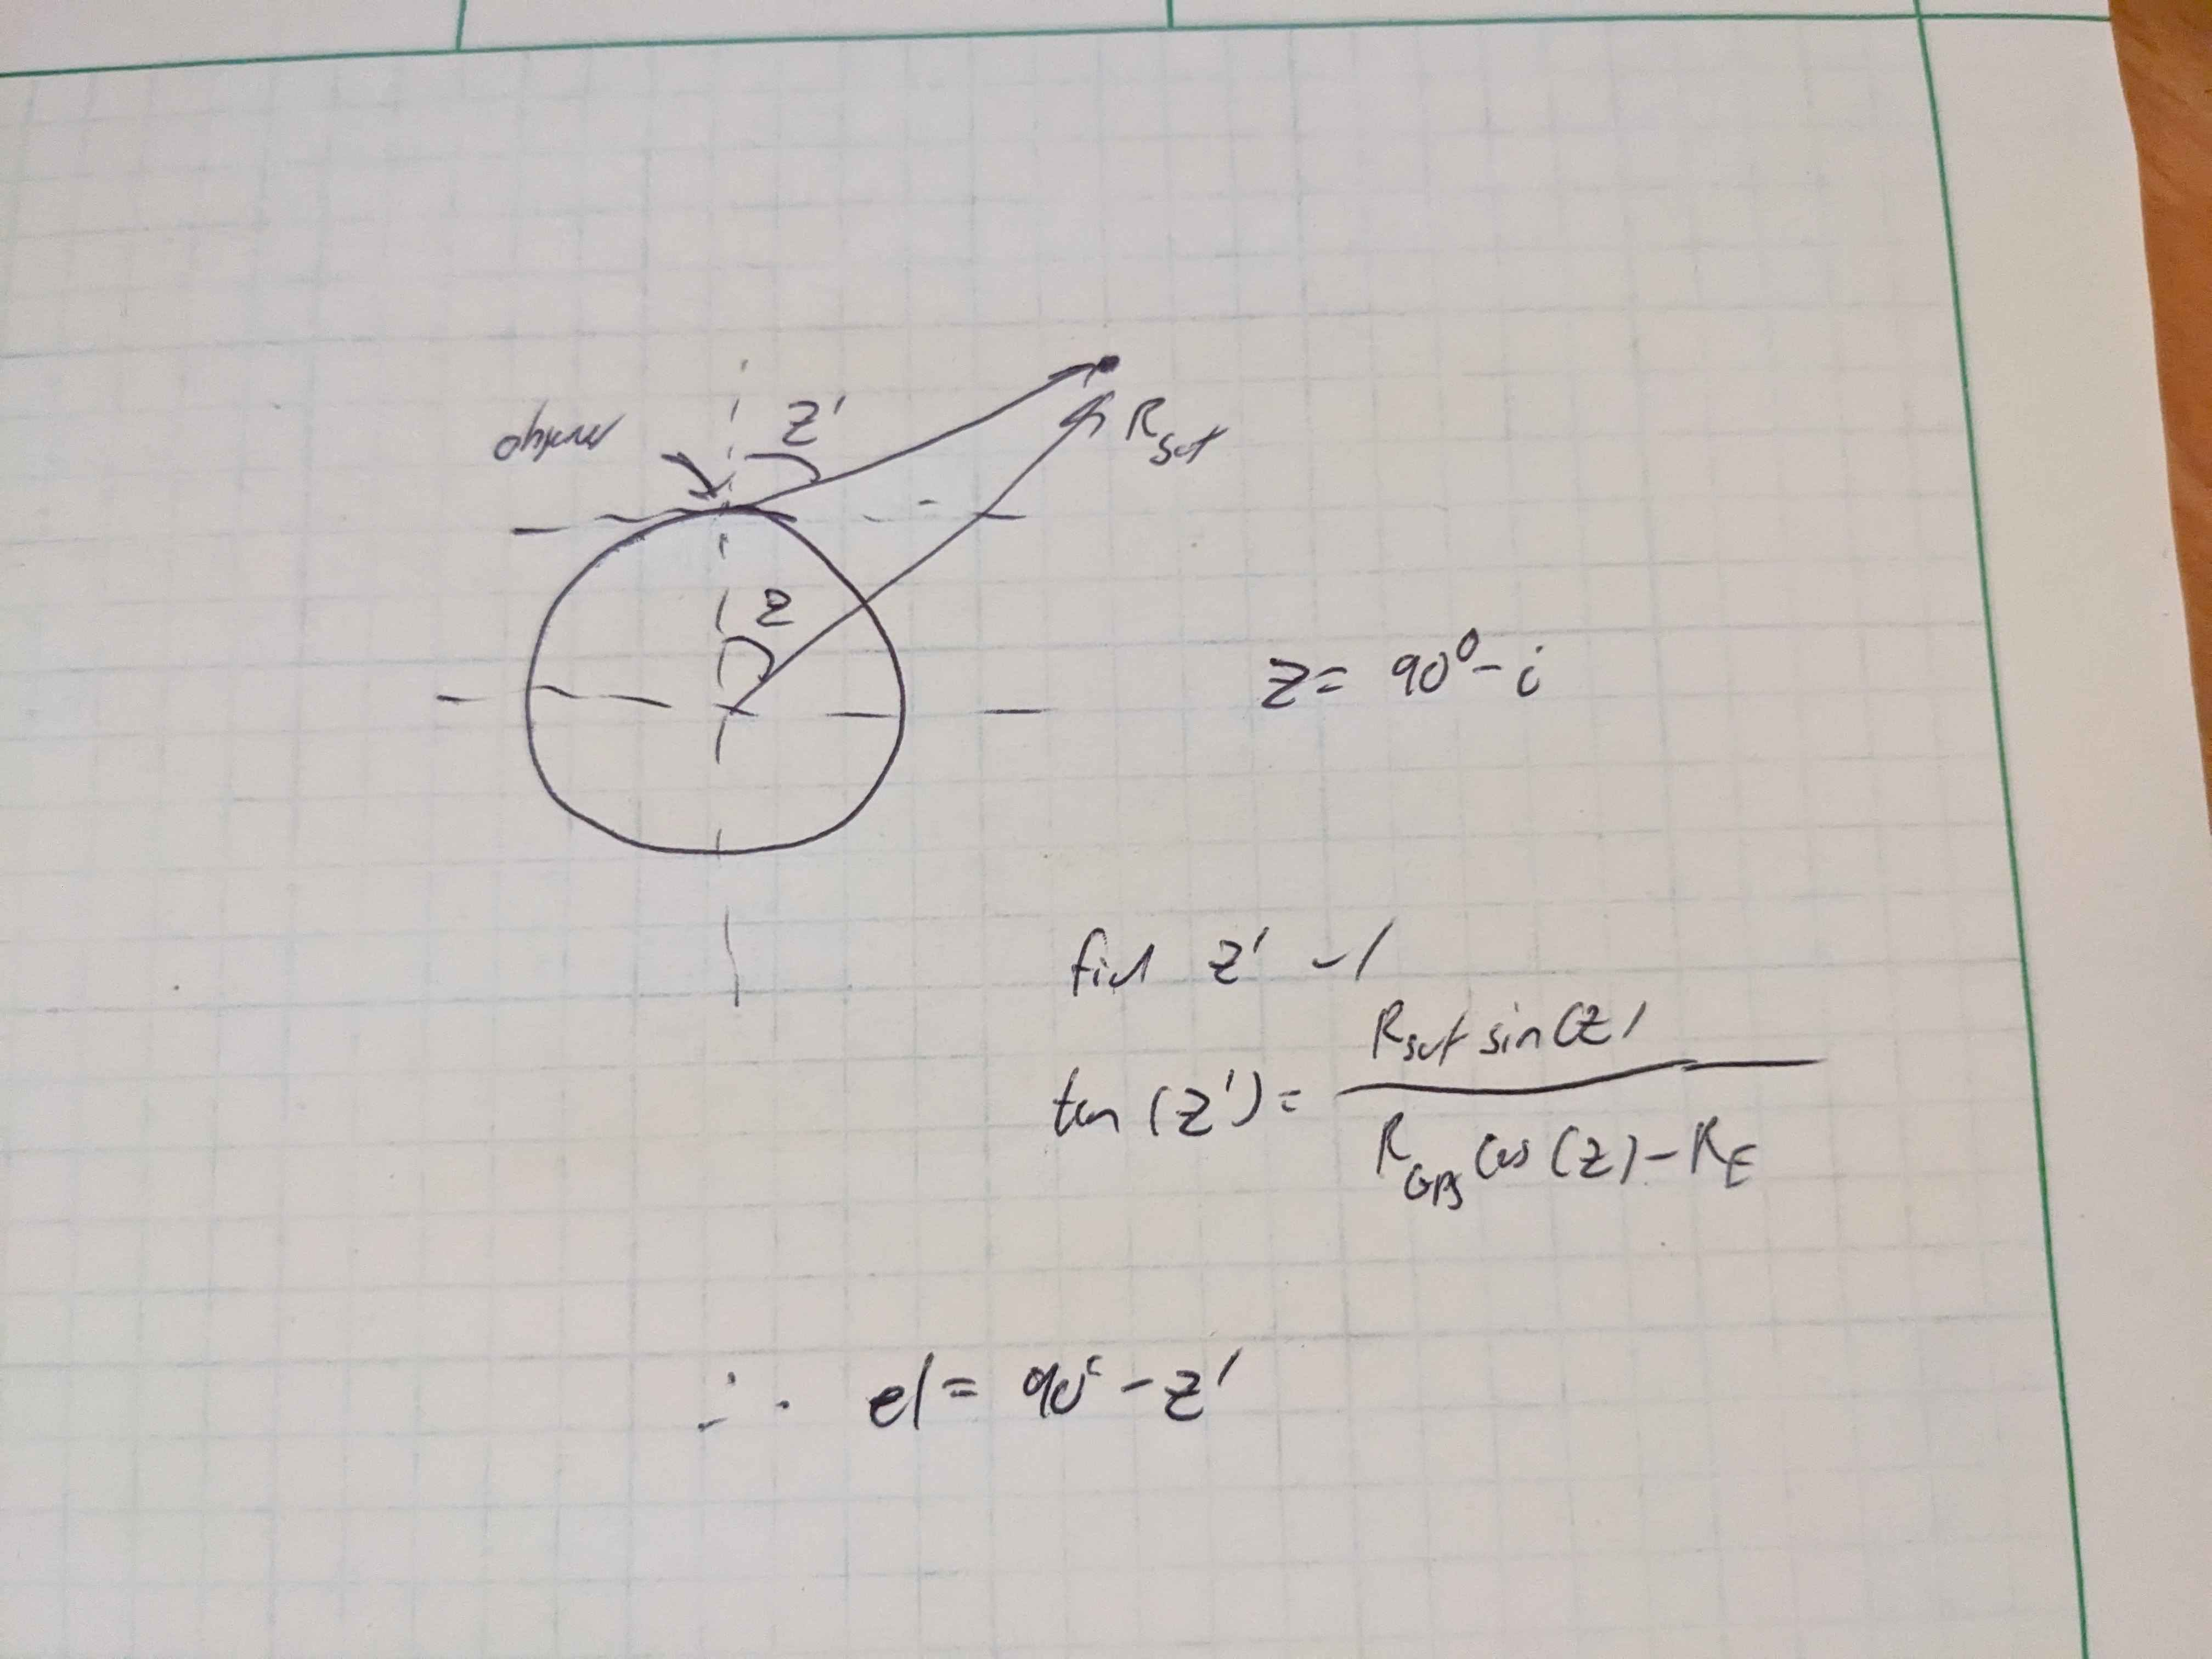
\includegraphics[width=0.6\textwidth]{north_pole_visability.jpg}
    \caption{North Pole Visibility Diagram}
    \label{fig:north_pole_visability}
\end{figure}

\hspace*{2em}Visibility can be calculated based on what can be seen in Figure \ref{fig:north_pole_visability}, and the equation,
\begin{gather*}
\tan{z^\prime} = \frac{R_{sat}\sin{z}}{R_{sat}\cos{z} - R_E} \\
z = 90^\circ - i \\
el = 90^\circ - z^\prime
\end{gather*}
\hspace*{2em}We can use $\arctan$ to find $z^\prime$ for LEO and GPS, we can then find their respective elevations.
\begin{gather*}
\boxed{el_{LEO NorthPole} = -6.9^\circ}\\
\boxed{el_{GPS NorthPole} = 45.3^\circ}
\end{gather*}
\hspace*{2em}This means that through the entire orbit of the LEO sat, an observer on the North Pole would never be able to observe it as the maximum elevation that it would ever reach relative to the North Pole would be below the horizon. By contrast, the GPS satellite will be observed though at a maximum of $45.3^\circ$ in elevation, essentially only half of the sky.

\newpage
\section*{Problem 2:}
\subsection*{(a.)}


\subsection*{(b.)}

\subsection*{(c.)}

\newpage
\section*{Problem 3:}
\subsection*{(a.)}

\subsection*{(b.)}

\subsection*{(c.)}

\subsection*{(d.)}


\end{document}
